\begin{figure}[t]
  \centering
  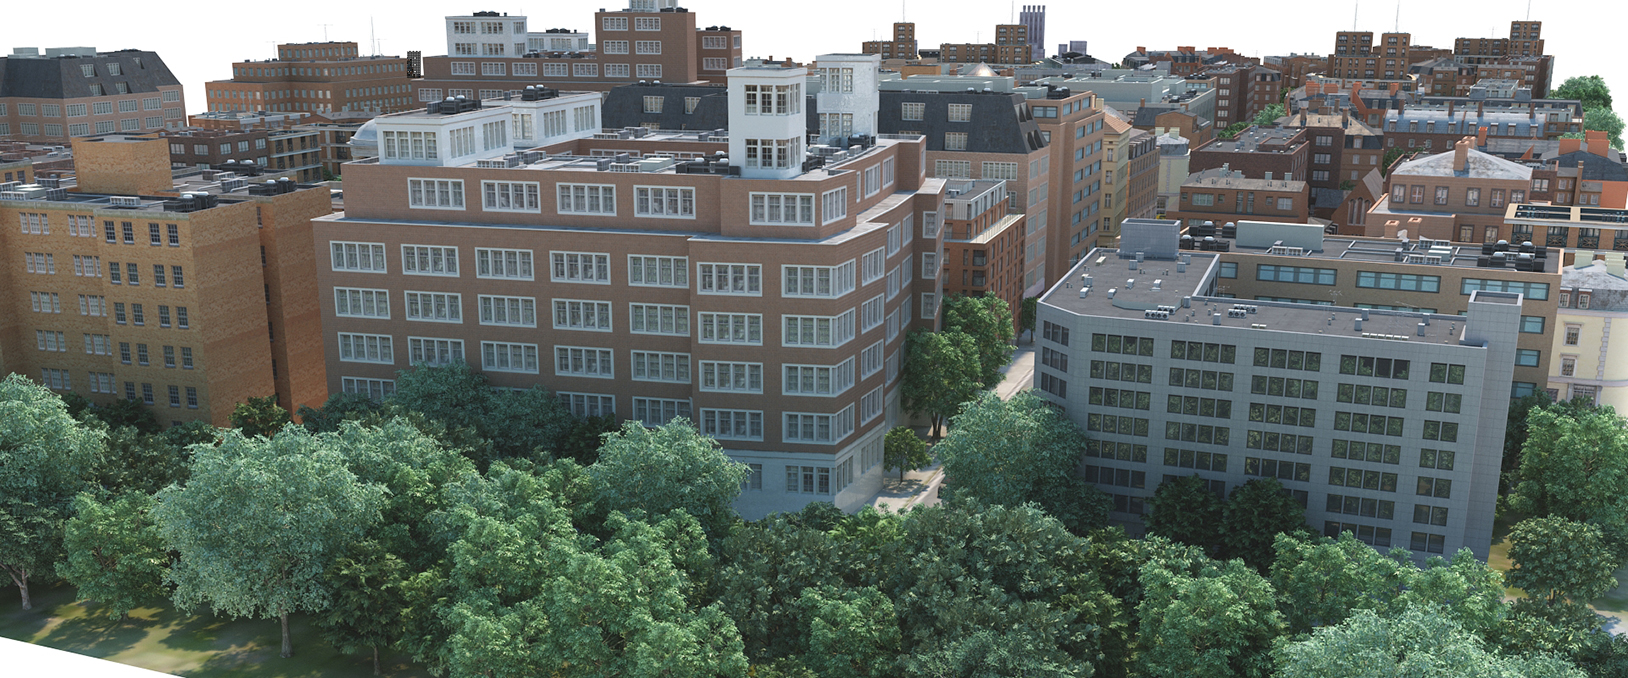
\includegraphics[width=\columnwidth]{densecity.jpg}
  \caption{Urban model: 100 million triangles, 12 GB. Using our method the walkthrough rendering performance for this model was significantly improved over existing methods. }
  \label{fig:model3}
\end{figure}

\section{Introduction}

%\subsection{Walkthrough Rendering}

In typical walkthrough systems, data sets consisting of hundreds of millions of
triangles and many gigabytes of associated data (e.g. walking through a virtual
city) are quite common. Rendering such massive amounts of data requires
out-of-core rendering algorithms that bring only the required data for
rendering into main memory from secondary storage. In this process, in addition
to the rendering speed, the data fetch speed also becomes critical for
achieving interactivity, especially when we handle large-scale data. In
general, data fetch speed depends on data seek time and data transfer time.
Transfer time depends only on the amount of data that is transferred. Seek time
is the time taken to locate the beginning of the required data in the storage
device and depends on different factors depending on the storage medium. \\
\\
For a hard disk drive (HDD), its seek time depends on the speed of rotating the
disk,
and the relative placement of the data units with respect to each other, also
called the data layout~\cite{Rizvi10}. For a solid state drive (SSD), this seek
time is usually a small constant and is independent of the location of the data
with respect to each other~\cite{SSD_perf08}. An earlier work utilized this
difference between SSD and HDD, and designed a data layout tailored for using
SSDs with the walkthrough application~\cite{ssdpaper}. There have been many
other techniques utilizing SSDs for various applications~\cite{FlashVM09}. SSD,
unfortunately, is not the perfect data storage and has its own technical
problems, including limited number of data overwrites allowed, high cost, and
limited capacity~\cite{Rizvi10}.  \\
\\
On the other hand, the HDD technology -- including disk technologies such as
CDs, DVDs, and Blu-ray discs -- has become quite reliable and inexpensive
thanks to their extensive verifications and testing, and is thus in widespread
use.  Even for massive data sets HDDs are still and will be
the preferred medium of storage for the foreseeable future~\cite{Rizvi10},
mainly
because of its stability and low cost per unit. As an example, according
to~\cite{pcmagarticle}, as of 2014, an HDD can cost \$0.08 per GB, while an SDD
can cost \$0.60 per GB. As a result, optimizing components of walkthrough
systems with HDDs is critical. In particular, addressing the seek time, the
main bottleneck of accessing data from HDDs, remains the main challenge for
interactive rendering of massive data sets. \\
%In this paper, we leverage the
%inexpensive nature of HDDs to store redundant copies of data in order to reduce
%the seek time. 
\\
There are generally two types of disk-based secondary storage devices. For devices with constant linear velocity (CLV), for example, Blu-ray, the seek speed is linearly dependent on the seek distance, the physical distance between data units. For devices with constant angular velocity (CAV), such as modern CDs and DVDs, most of the data is stored along the rim to enable faster seek time, so we can assume the seek speed is almost linear which respect to seek distance. In both cases, minimizing seek distance generally produces a data layout that will minimize seek time. \\
\\
In this paper, we leverage the inexpensive nature of HDDs to store redundant
copies of data in order to reduce the seek time. Adding redundancy in order to
improve the data access time is a classic approach, e.g.,
RAID~\cite{Patterson88}.  We are also not the first to consider redundancy for
walkthrough applications.  Redundancy based data layouts to reduce the seek
time were introduced in a recent work~\cite{singleseeklayout}, in which the
number of seeks for every access was reduced to at most one unit. However, in
order to achieve this nice property, the redundancy factor -- the ratio between
the size of the data after using redundancy to the original size of the data --
was
prohibitively high around 80. \\
\\
Another recent work \cite{optimizingredundancy} took the data transfer time, seek time,
and redundancy, and proposed a linear programming approach to optimize the data
transfer and seek time in order to satisfy the total data fetch time
constraint. In the process, redundancy was a hidden variable that was
minimized. Unfortunately, this approach does not directly model redundancy or
seek time, and thus can have unnecessary data blocks and unrealistic seek
times.
%\YOON{I think that we need to compare the current work against this work in a way in the .}. 

%\subsection{Main Contributions}
{\bf Main contributions:}
In this paper, we propose a model for seek time based on the actual
number of units
between the data blocks in the linear data layout. Using this model, and given
the spatial proximity of the data set for a walkthrough application, we develop
an algorithm to duplicate data blocks strategically to maximize the reduction
in the seek time, while keeping the redundancy factor within the user defined
bound. We will show that our greedy solution can generate both the extreme cases
of data layout with redundancy, namely the maximum redundancy case
(a layout where seek time is at most one) and the no-redundancy case (a simple
cache oblivious mesh layout with a potentially high seek time), as well as
reasonable solutions for redundancy factor constraints in between the extremes.
We show that the
implementation of our algorithm significantly reduces average delay between
frames and noticeably improves the consistency of performance and
interactivity.